\section{Tool Flow}
Figure~\ref{fig:flow} delineates the flow diagram of \textit{MXCplore}. 
The user starts by invoking the \textbf{\textit{mcxplore.sh}} script with the desired model. 
If the model was the \textbf{noMChk} one, the tool invokes the \textbf{\textit{MCXplore\_noMChk.pl}} script. 
\textbf{\textit{MCXplore\_noMChk.pl}} executes the following procedure:
\begin{enumerate}
\item Call \textbf{\textit{ReadConfiguration.pl}} to read the user configurations and extract the address segments. 

\item Generate the request address by invoking \textbf{\textit{AddressGeneration.pl}} and generate the request type by invoking \textbf{\textit{TypeGeneration.pl}} 

\item Print the request by calling \textbf{print\_request()} method in \textbf{\textit{GenerateTest.pl}} 
\item Repeat steps 2 and 3 for the number of requests specified by the user 
\end{enumerate} 

On the other hand, if the user specified the \textbf{CMDmdl} model, the tool invokes  the \textbf{\textit{MCXplore\_REQmdl.sh}} script. 
\textbf{\textit{MCXplore\_REQmdl.sh}} executes the following procedure: 

\begin{enumerate}
\item Run the NuSMV model checker on the CMDmdl.smv model. This step produces the test template (\textbf{\textit{CMDmdl.bmc}}), which is the path produced by bounded model checking. 

\item Call \textbf{\textit{CMDmdl\_parser.pl}} to parse the test template. The parser first reads the user configurations (Specifically the address mapping and the model-independent configurations). 

\item For each state in the template, Generate a request and print it in the test output file by calling the \textbf{generate\_request()} method in \textbf{\textit{GeenrateTest.pl}} script.
\end{enumerate} 

For the \textbf{REQmdl} model, \textit{MCXplore} deploys a similar procedure on the corresponding scripts for that model.





\begin{figure*}[tp]
\begin{center}
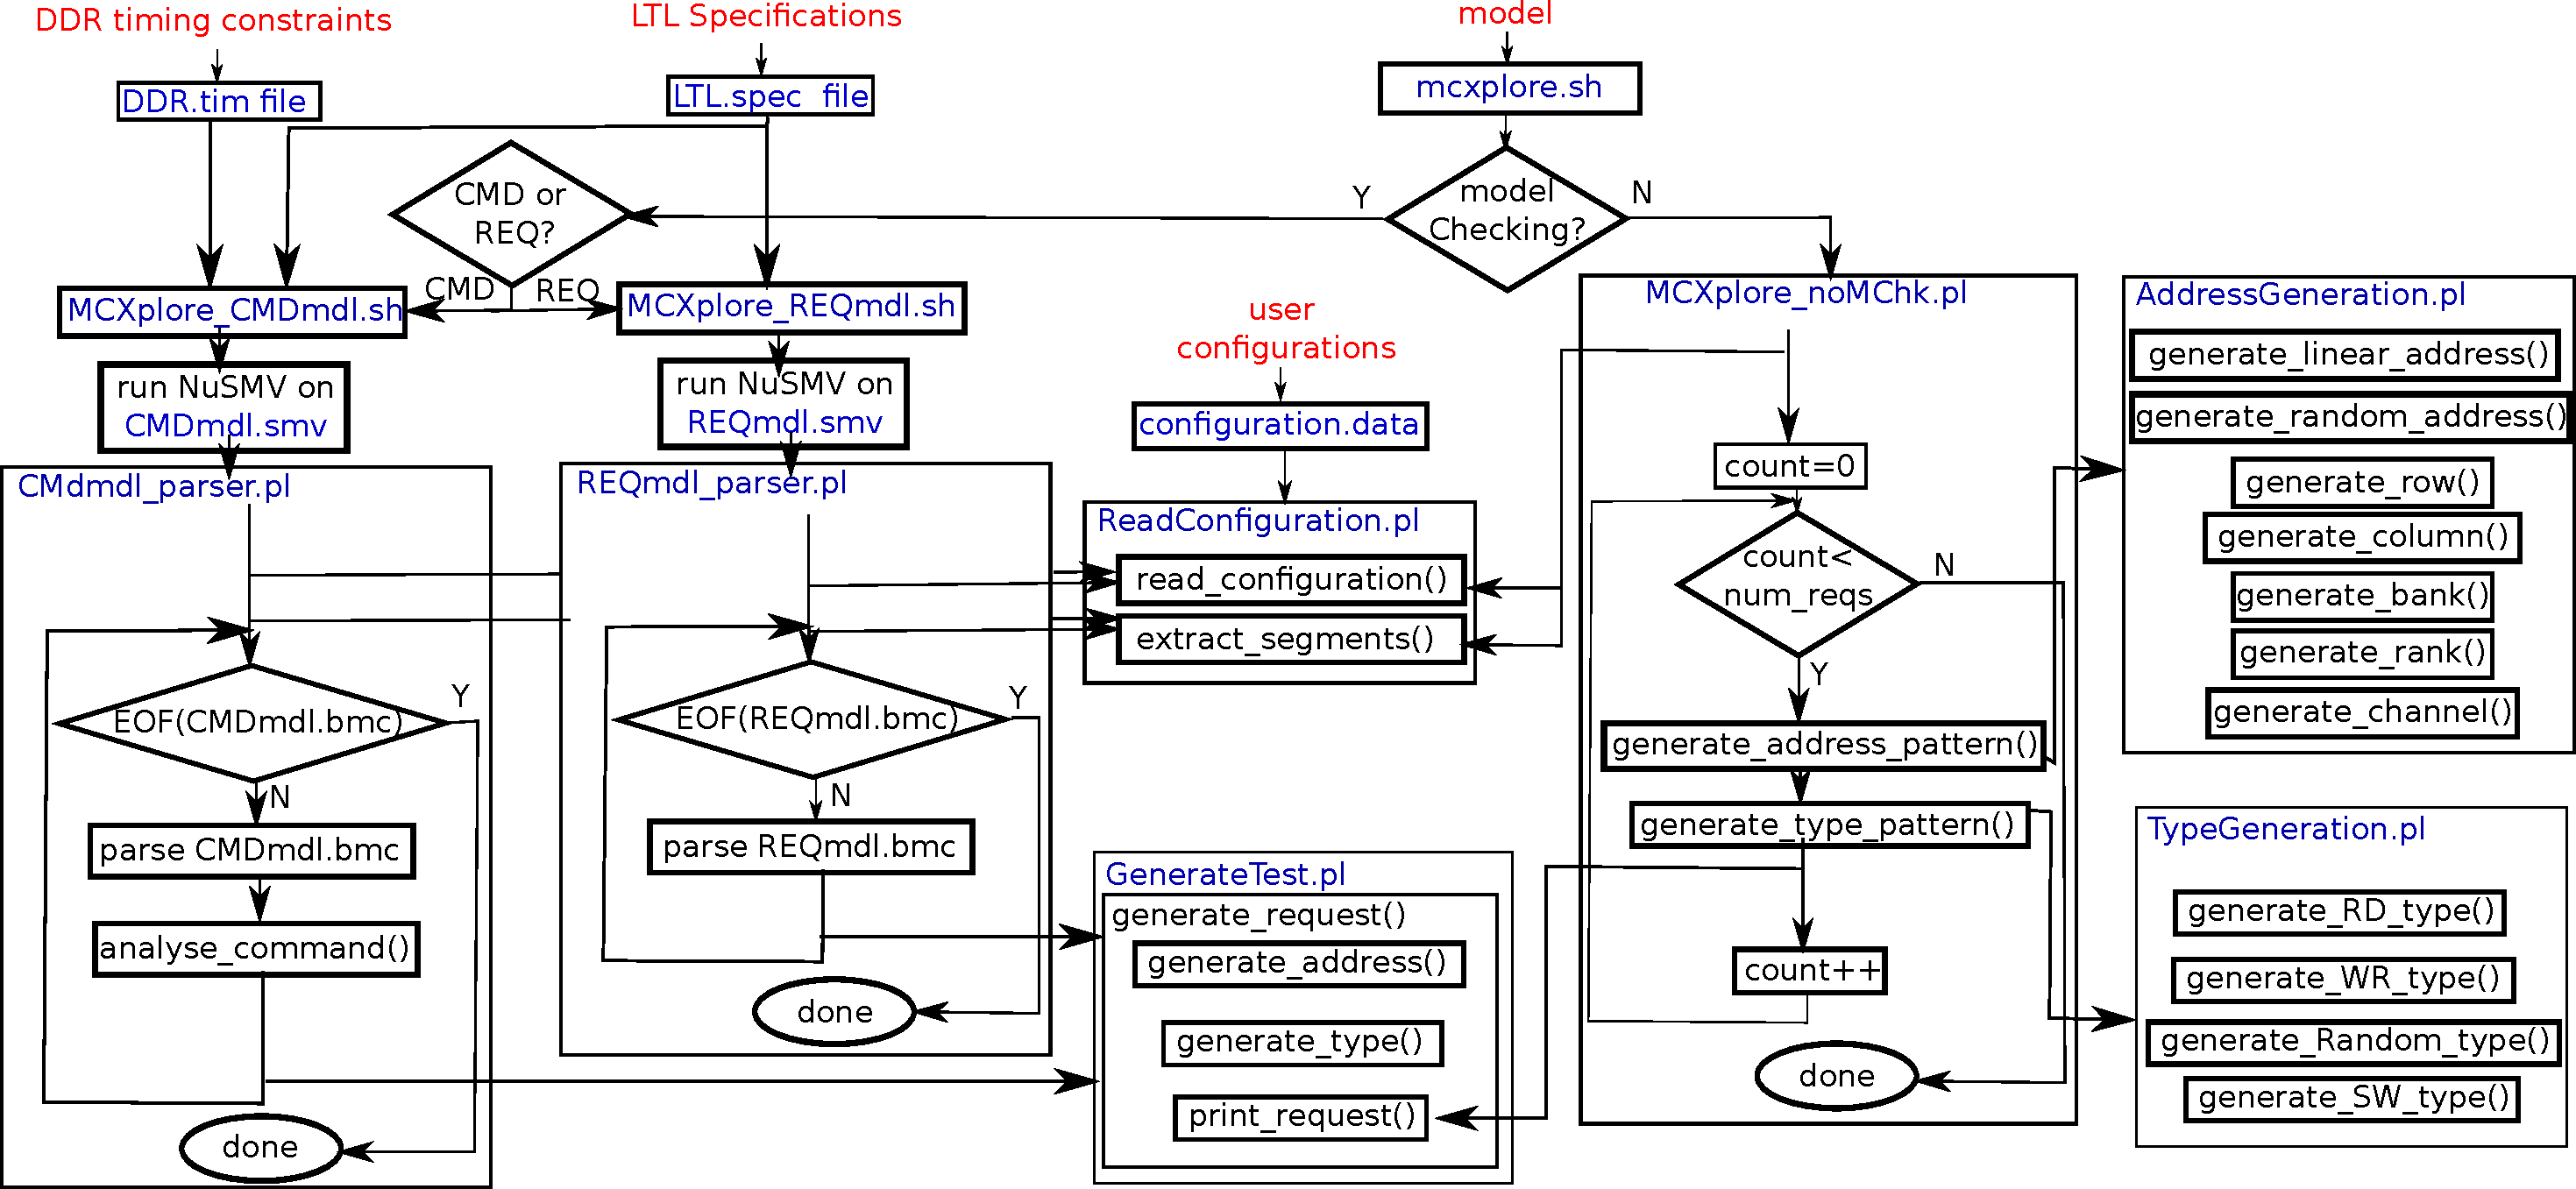
\includegraphics[scale=0.35]{MCXplore_flow.pdf}
\end{center}
\caption{MCXplore tool flow.~\label{fig:flow}}
\end{figure*}